
%% bare_conf.tex
%% V1.4b
%% 2015/08/26
%% by Michael Shell
%% See:
%% http://www.michaelshell.org/
%% for current contact information.
%%
%% This is a skeleton file demonstrating the use of IEEEtran.cls
%% (requires IEEEtran.cls version 1.8b or later) with an IEEE
%% conference paper.
%%
%% Support sites:
%% http://www.michaelshell.org/tex/ieeetran/
%% http://www.ctan.org/pkg/ieeetran
%% and
%% http://www.ieee.org/

%%*************************************************************************
%% Legal Notice:
%% This code is offered as-is without any warranty either expressed or
%% implied; without even the implied warranty of MERCHANTABILITY or
%% FITNESS FOR A PARTICULAR PURPOSE!
%% User assumes all risk.
%% In no event shall the IEEE or any contributor to this code be liable for
%% any damages or losses, including, but not limited to, incidental,
%% consequential, or any other damages, resulting from the use or misuse
%% of any information contained here.
%%
%% All comments are the opinions of their respective authors and are not
%% necessarily endorsed by the IEEE.
%%
%% This work is distributed under the LaTeX Project Public License (LPPL)
%% ( http://www.latex-project.org/ ) version 1.3, and may be freely used,
%% distributed and modified. A copy of the LPPL, version 1.3, is included
%% in the base LaTeX documentation of all distributions of LaTeX released
%% 2003/12/01 or later.
%% Retain all contribution notices and credits.
%% ** Modified files should be clearly indicated as such, including  **
%% ** renaming them and changing author support contact information. **
%%*************************************************************************


% *** Authors should verify (and, if needed, correct) their LaTeX system  ***
% *** with the testflow diagnostic prior to trusting their LaTeX platform ***
% *** with production work. The IEEE's font choices and paper sizes can   ***
% *** trigger bugs that do not appear when using other class files.       ***                          ***
% The testflow support page is at:
% http://www.michaelshell.org/tex/testflow/



\documentclass[conference]{IEEEtran}
% Some Computer Society conferences also require the compsoc mode option,
% but others use the standard conference format.
%
% If IEEEtran.cls has not been installed into the LaTeX system files,
% manually specify the path to it like:
% \documentclass[conference]{../sty/IEEEtran}





% Some very useful LaTeX packages include:
% (uncomment the ones you want to load)


% *** MISC UTILITY PACKAGES ***
%
%\usepackage{ifpdf}
% Heiko Oberdiek's ifpdf.sty is very useful if you need conditional
% compilation based on whether the output is pdf or dvi.
% usage:
% \ifpdf
%   % pdf code
% \else
%   % dvi code
% \fi
% The latest version of ifpdf.sty can be obtained from:
% http://www.ctan.org/pkg/ifpdf
% Also, note that IEEEtran.cls V1.7 and later provides a builtin
% \ifCLASSINFOpdf conditional that works the same way.
% When switching from latex to pdflatex and vice-versa, the compiler may
% have to be run twice to clear warning/error messages.






% *** CITATION PACKAGES ***
%
%\usepackage{cite}
% cite.sty was written by Donald Arseneau
% V1.6 and later of IEEEtran pre-defines the format of the cite.sty package
% \cite{} output to follow that of the IEEE. Loading the cite package will
% result in citation numbers being automatically sorted and properly
% "compressed/ranged". e.g., [1], \cite{seznec2007tage}, \cite{calder1997evidence}, \cite{lee1995branch}, \cite{jimenez2001dynamic}, \cite{jimenez2003fast} without using
% cite.sty will become [1], \cite{calder1997evidence}, \cite{jimenez2001dynamic}--\cite{lee1995branch}, \cite{seznec2007tage} using cite.sty. cite.sty's
% \cite will automatically add leading space, if needed. Use cite.sty's
% noadjust option (cite.sty V3.8 and later) if you want to turn this off
% such as if a citation ever needs to be enclosed in parenthesis.
% cite.sty is already installed on most LaTeX systems. Be sure and use
% version 5.0 (2009-03-20) and later if using hyperref.sty.
% The latest version can be obtained at:
% http://www.ctan.org/pkg/cite
% The documentation is contained in the cite.sty file itself.






% *** GRAPHICS RELATED PACKAGES ***
%
\ifCLASSINFOpdf
  % \usepackage[pdftex]{graphicx}
  % declare the path(s) where your graphic files are
  % \graphicspath{{../pdf/}{../jpeg/}}
  % and their extensions so you won't have to specify these with
  % every instance of \includegraphics
  % \DeclareGraphicsExtensions{.pdf,.jpeg,.png}
\else
  % or other class option (dvipsone, dvipdf, if not using dvips). graphicx
  % will default to the driver specified in the system graphics.cfg if no
  % driver is specified.
  % \usepackage[dvips]{graphicx}
  % declare the path(s) where your graphic files are
  % \graphicspath{{../eps/}}
  % and their extensions so you won't have to specify these with
  % every instance of \includegraphics
  % \DeclareGraphicsExtensions{.eps}
\fi
\usepackage{algorithm}
\usepackage{algpseudocode}
\usepackage{amsmath}
\usepackage{amsmath,amssymb,amsthm,latexsym,paralist, booktabs}
\usepackage{url}
\usepackage[pdftex]{graphicx}
% default pic path
\usepackage{bm}
\usepackage{mathtools}
\let\oldvec\vec
\renewcommand{\vec}[1]{\oldvec{\mathit{#1}}}
\newcommand{\mat}[1]{\mathbf{#1}} % undergraduate algebra version
\newcommand{\parallelsum}{\mathbin{\!/\mkern-5mu/\!}}
\graphicspath{{pics/}}
\usepackage{subfigure}

\usepackage{listings}
\usepackage{color} %red, green, blue, yellow, cyan, magenta, black, white
\definecolor{mygreen}{RGB}{28,172,0} % color values Red, Green, Blue
\definecolor{mylilas}{RGB}{170,55,241}

%\newcommand{\mat}[1]{\bm{\mathit{#1}}}




% *** Do not adjust lengths that control margins, column widths, etc. ***
% *** Do not use packages that alter fonts (such as pslatex).         ***
% There should be no need to do such things with IEEEtran.cls V1.6 and later.
% (Unless specifically asked to do so by the journal or conference you plan
% to submit to, of course. )


% correct bad hyphenation here
\hyphenation{op-tical net-works semi-conduc-tor}


\begin{document}
\lstset{language=Matlab,%
    %basicstyle=\color{red},
    breaklines=true,%
    morekeywords={matlab2tikz},
    keywordstyle=\color{blue},%
    morekeywords=[2]{1}, keywordstyle=[2]{\color{black}},
    identifierstyle=\color{black},%
    stringstyle=\color{mylilas},
    commentstyle=\color{mygreen},%
    showstringspaces=false,%without this there will be a symbol in the places where there is a space
    numbers=left,%
    numberstyle={\tiny \color{black}},% size of the numbers
    numbersep=9pt, % this defines how far the numbers are from the text
    emph=[1]{for,end,break},emphstyle=[1]\color{red}, %some words to emphasise
    %emph=[2]{word1,word2}, emphstyle=[2]{style},    
}
%
% paper title
% Titles are generally capitalized except for words such as a, an, and, as,
% at, but, by, for, in, nor, of, on, or, the, to and up, which are usually
% not capitalized unless they are the first or last word of the title.
% Linebreaks \\ can be used within to get better formatting as desired.
% Do not put math or special symbols in the title.
\title{CSCE 643 Multi-View Geometry CV\\
Project II}


% author names and affiliations
% use a multiple column layout for up to three different
% affiliations

% conference papers do not typically use \thanks and this command
% is locked out in conference mode. If really needed, such as for
% the acknowledgment of grants, issue a \IEEEoverridecommandlockouts
% after \documentclass

% for over three affiliations, or if they all won't fit within the width
% of the page, use this alternative format:
%
%\author{\IEEEauthorblockN{Michael Shell\IEEEauthorrefmark{1},
%Homer Simpson\IEEEauthorrefmark{2},
%James Kirk\IEEEauthorrefmark{3},
%Montgomery Scott\IEEEauthorrefmark{3} and
%Eldon Tyrell\IEEEauthorrefmark{4}}
%\IEEEauthorblockA{\IEEEauthorrefmark{1}School of Electrical and Computer Engineering\\
%Georgia Institute of Technology,
%Atlanta, Georgia 30332--0250\\ Email: see http://www.michaelshell.org/contact.html}
%\IEEEauthorblockA{\IEEEauthorrefmark{2}Twentieth Century Fox, Springfield, USA\\
%Email: homer@thesimpsons.com}
%\IEEEauthorblockA{\IEEEauthorrefmark{3}Starfleet Academy, San Francisco, California 96678-2391\\
%Telephone: (800) 555--1212, Fax: (888) 555--1212}
%\IEEEauthorblockA{\IEEEauthorrefmark{4}Tyrell Inc., 123 Replicant Street, Los Angeles, California 90210--4321}}




% use for special paper notices
%\IEEEspecialpapernotice{(Invited Paper)}




% make the title area
\maketitle
\begin{abstract}
In this project, we explore and investigate different approaches for estimation in 2D projective transformation. In total, we implemented 3 approaches for finding the homography transformation between two different images, Direct Linear Transformation (DLT), normalized DLT and DLT with Sampson error minimization. This paper mainly focuses on the mathematical foundations for those methodologies used in our implementation and presents the results through combining two images into one panorama to validate the correctness of our approach. We can see clearly that with the advancement of our approach, the sampson error is gradually reduced (though there are few differences we can notice between those image panorama results).
\end{abstract}
% As a general rule, do not put math, special symbols or citations
% in the abstract

% no keywords




% For peer review papers, you can put extra information on the cover
% page as needed:
% \ifCLASSOPTIONpeerreview
% \begin{center} \bfseries EDICS Category: 3-BBND \end{center}
% \fi
%
% For peerreview papers, this IEEEtran command inserts a page break and
% creates the second title. It will be ignored for other modes.
\IEEEpeerreviewmaketitle


\section{Calibrate Lens Distortion}
A basic assumption in camera geometry study is that a linear model is an accurate model of the imaging process, i.e., world point, image point and optical center point are collinear and world lines are imaged as lines and so on. However, this might not be true for real lens in the world. Radial distortion is a typical deviation that real lens might have, we need to correct image measurements to those that should be obtained under a perfect linear camera action.

\subsection{Problem Formulation}
Suppose $(\tilde{x}, \tilde{y})$ is the ideal image position that obeys linear projection (under perfect lens settings), $(x_d, y_d)$ to be the actual image position after the effects of radial distortion, $\tilde{r} = \sqrt{\tilde{x^2} + \tilde{y^2}}$ is the radial distance from the center of radial distortion, $L(\tilde{r})$ is a function of radius $\tilde{r}$ as the distortion factor. 

For the coordinates of point under non-distorted pinhole projection $(\tilde{x}, \tilde{y})$ (in units of focal-length), we have:
\begin{equation}
	(\tilde{x}, \tilde{y}, 1)^T = [ I| \mat{0}] \mat{x}_{cam}
\end{equation}

where $\mat{x}_{cam}$ is the 3D point in camera coordinates and it is related to world coordinates as follows:
\begin{equation}
	\mat{x}_{cam} = \begin{bmatrix}
				R & -R\tilde{\mat{C}}\\
				0 & 1
			\end{bmatrix}
			\begin{pmatrix}
				X\\
				Y\\
				Z\\
				1
			\end{pmatrix}
			=\begin{bmatrix}
				R & -R\tilde{\mat{C}}\\
				0 & 1
			\end{bmatrix}\mat{x}
\end{equation}

Now we can easily model the radial distortion by introducing the function of $\tilde{r}$:
\begin{equation}
	\begin{pmatrix}
		x_d\\
		y_d
	\end{pmatrix}
	=L(\tilde{r})\begin{pmatrix}
		\tilde{x}\\
		\tilde{y}
	\end{pmatrix}
\end{equation}

If we dig into a single point coordinate $(x, y)$, we have:
\begin{equation}
\begin{split}
	\tilde{x} = x_c + L(r)(x-x_c)\\
	\tilde{y} = y_c + L(r)(y-y_c)
\end{split}
\end{equation}
where $(x_c, y_c)$ is center of the image, $(\tilde{x}, \tilde{y})$ is the coordinates after correcting radial distortion. Also be noticed that $r$ can is the radius from center of the image to the measured coordinates, which can be solved by:
\begin{equation}
	r^2 = (x-x_c)^2 + (y-y_c)^2
\end{equation}

\subsection{Distortion function and image center}
Now let's talk about the choice of function $L(r)$ and center of image $(x_c, y_c)$. According to the textbook, $L(r)$ is only defined for positive $r$ and $L(0) = 1$. We can use Taylor expansion as an approximation of the distortion function:
\begin{equation}
	L(r) = 1 + k_1r + k_2r^2 + k_3r^3 + \dots
\end{equation}

For image center $(x_c, y_c)$, we often use principal point though it might not reside in the exact same location. On choosing the distortion function for this project, we did a tradeoff consideration. Apparently if we have higher order Taylor expansion for distortion function, we can get better correcting results, however, as the camera we are actually using is really good (though it is a relatively old model, modern cameras are generally good enough and generates very little distortion), we decided to choose $L(r) = 1 + k_1r + k_2r^2$ as our distortion function.
The intuition behind this is that typically we choose higher order of distortion function as the degree of distortion increases, in our case the distortion is even ignorable thus we use a typical 2-order function to deal with our case.

\subsection{Distortion function minimization}
Similar as the minimization process we have done in the previous projects, here we need to minimize the geometric distance between predicted coordinates (by using $L(r)$) and measured coordinates. This can be done by exploiting the colinearity of points on the same line. In our project, we use the checker board image captured by our camera for lens distortion correction. The basic idea is that we can easily identify corner points on checker board and they naturally form parallel and perpendicular lines. If we determine a straight line using two corner points on the line, then all the other corner points along the line should be on the line if without radial distortion. Let's consider a simple scenario, suppose we have $\mat{A}, \mat{B}, \mat{D}$ on same line of a checker board, and the image center is $\mat{C}$, then we can do cross product to solve the crossing product of $\vec{AB}$ and $\vec{CD}$ to get $\mat{D}^{\prime} = \vec{AB}\times \vec{CD}$, due to the radial distortion we have $\mat{D} \neq \mat{D}^\prime$. If we apply $L(r)$ for the measured $D$ to get corrected coordinates $\hat{\mat{D}}$, we want to find a function that minimizes $d(\hat{\mat{D}}, \mat{D}^\prime)$. This is now reduced to a simple minimization problem of geometric distance like we did before, we can construct the corresponding error function based on discussions above and use non linear solver in MATLAB to get function $L(r)$ that does the required minimization.
%\begin{figure*}[!hbpt]
%  \subfigure[Original source image(the image we wanna transform)]{
%\label{fig1} %% label for second subfigure
%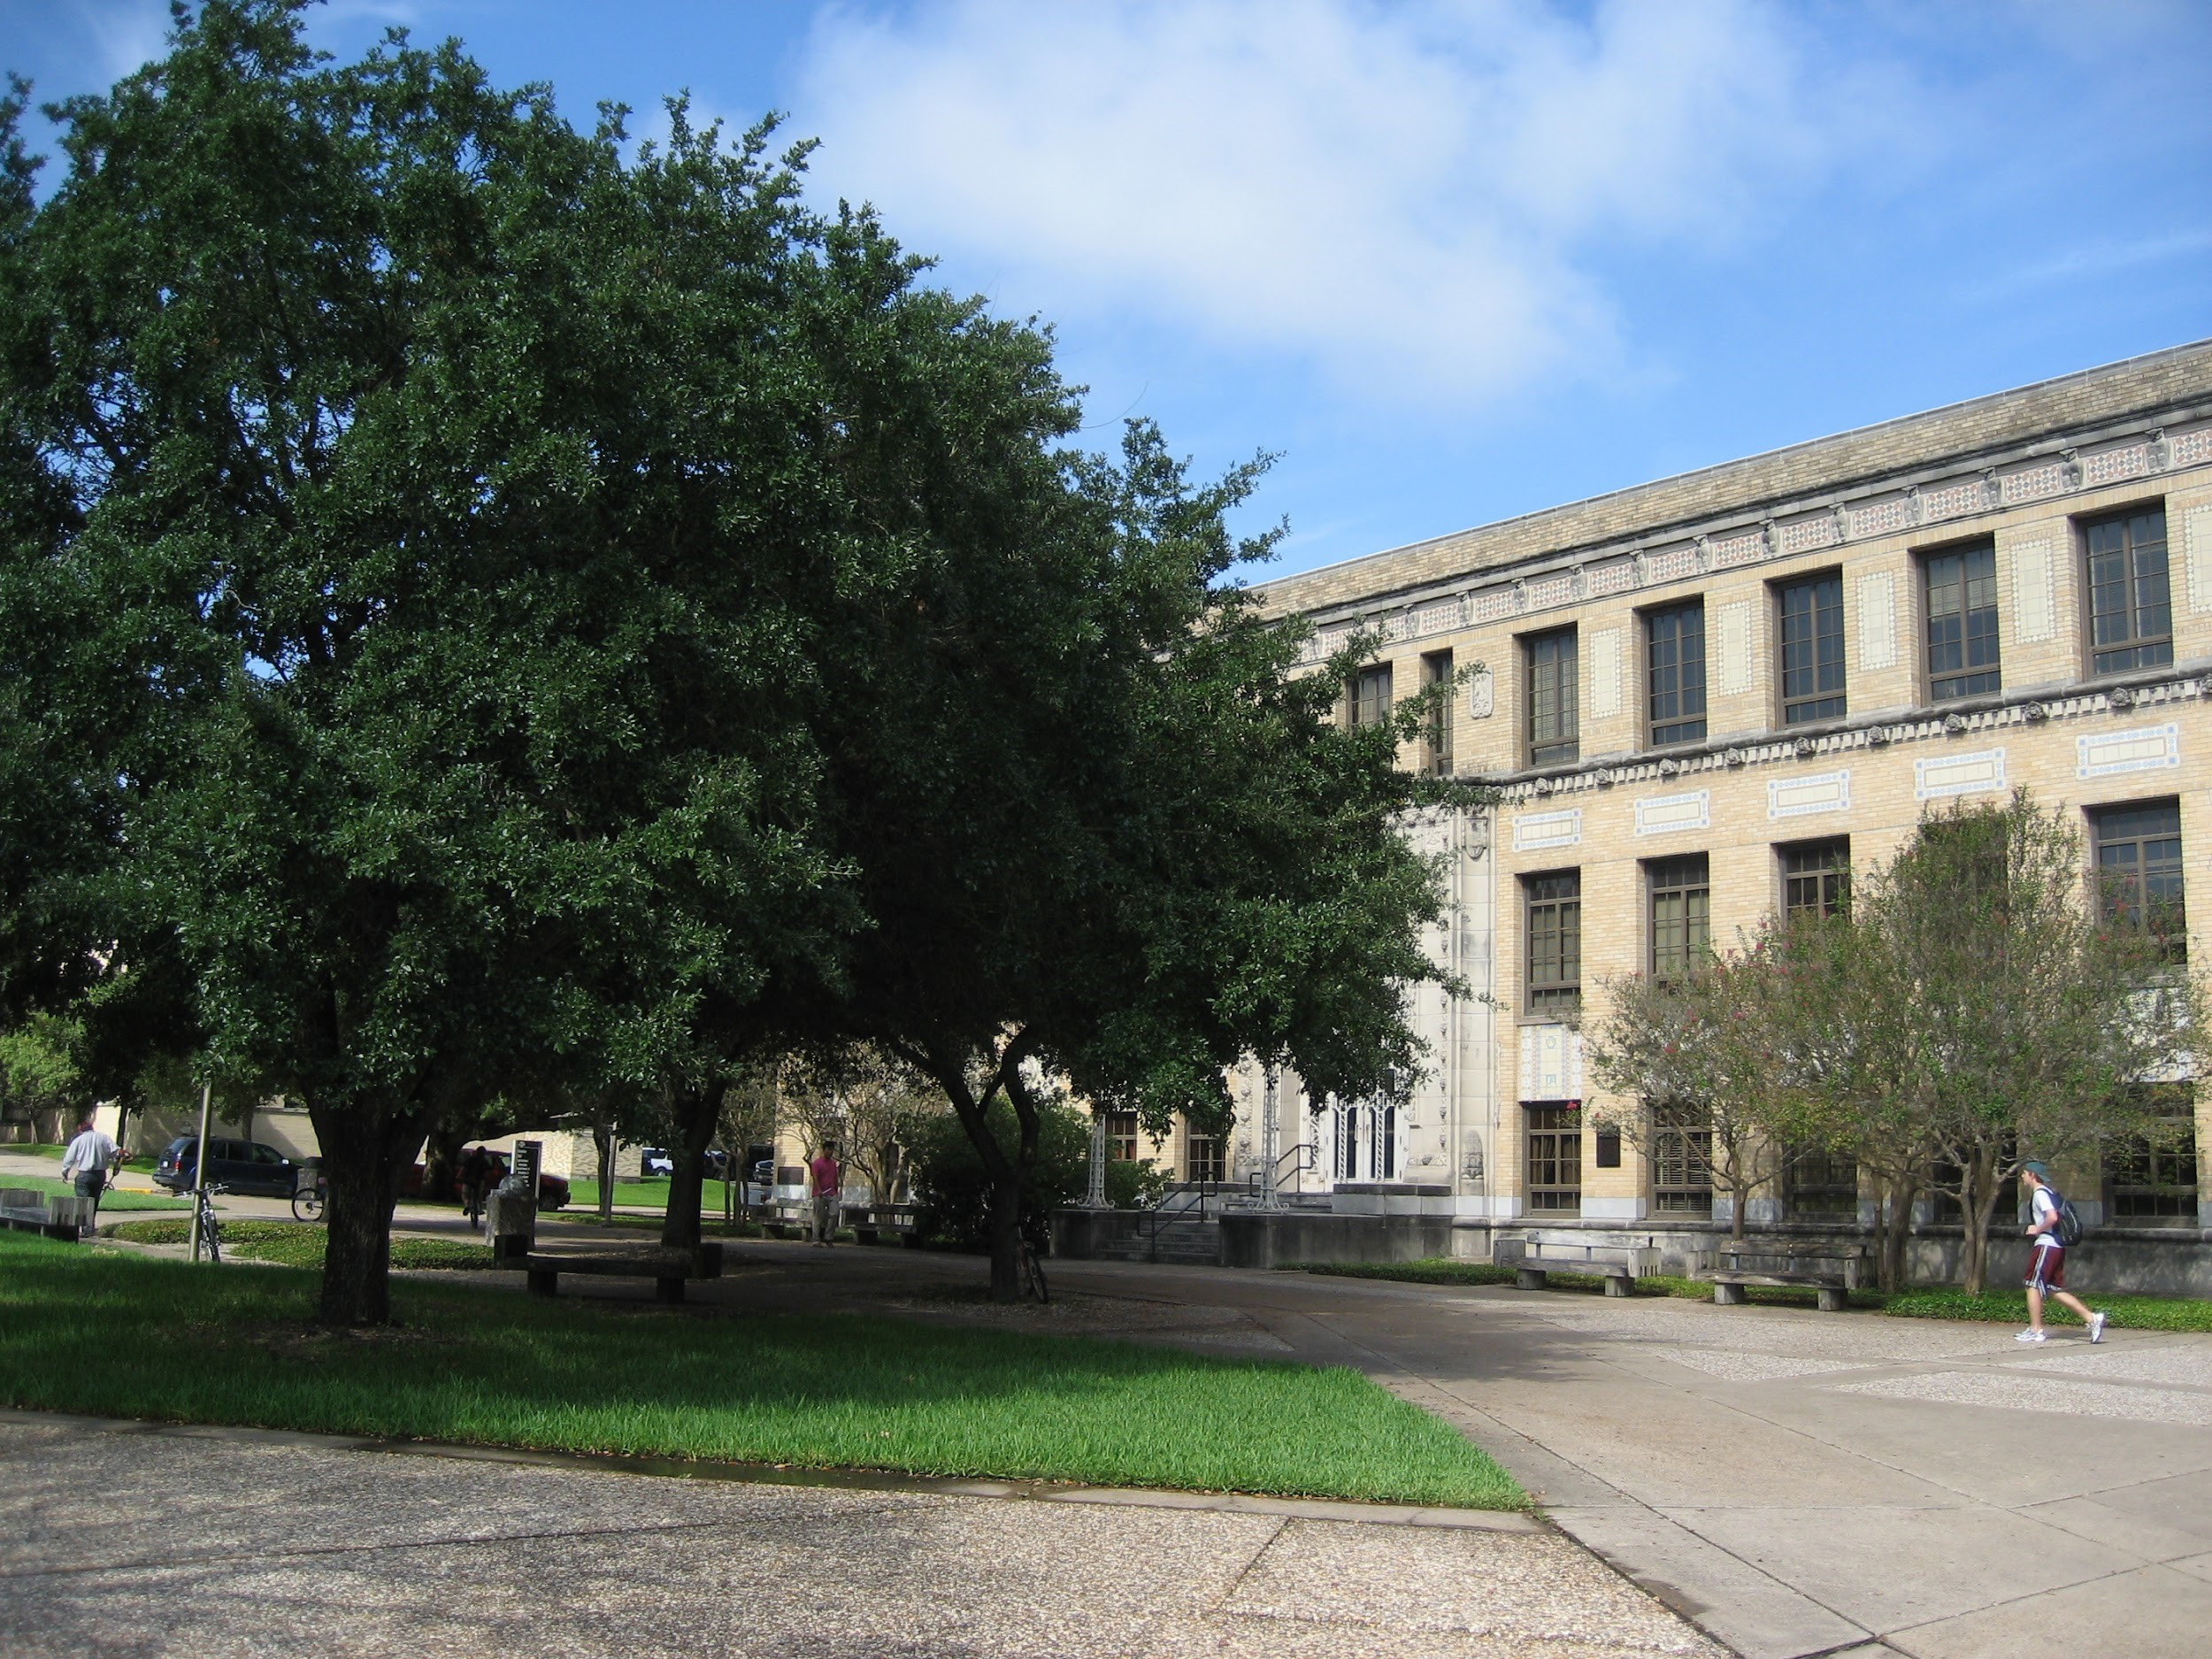
\includegraphics[width=0.49\linewidth]{fig_1.jpg}}
% \subfigure[The original target image(target image space we use for panorama)]{
%    \label{fig2} %% label for first subfigure
%    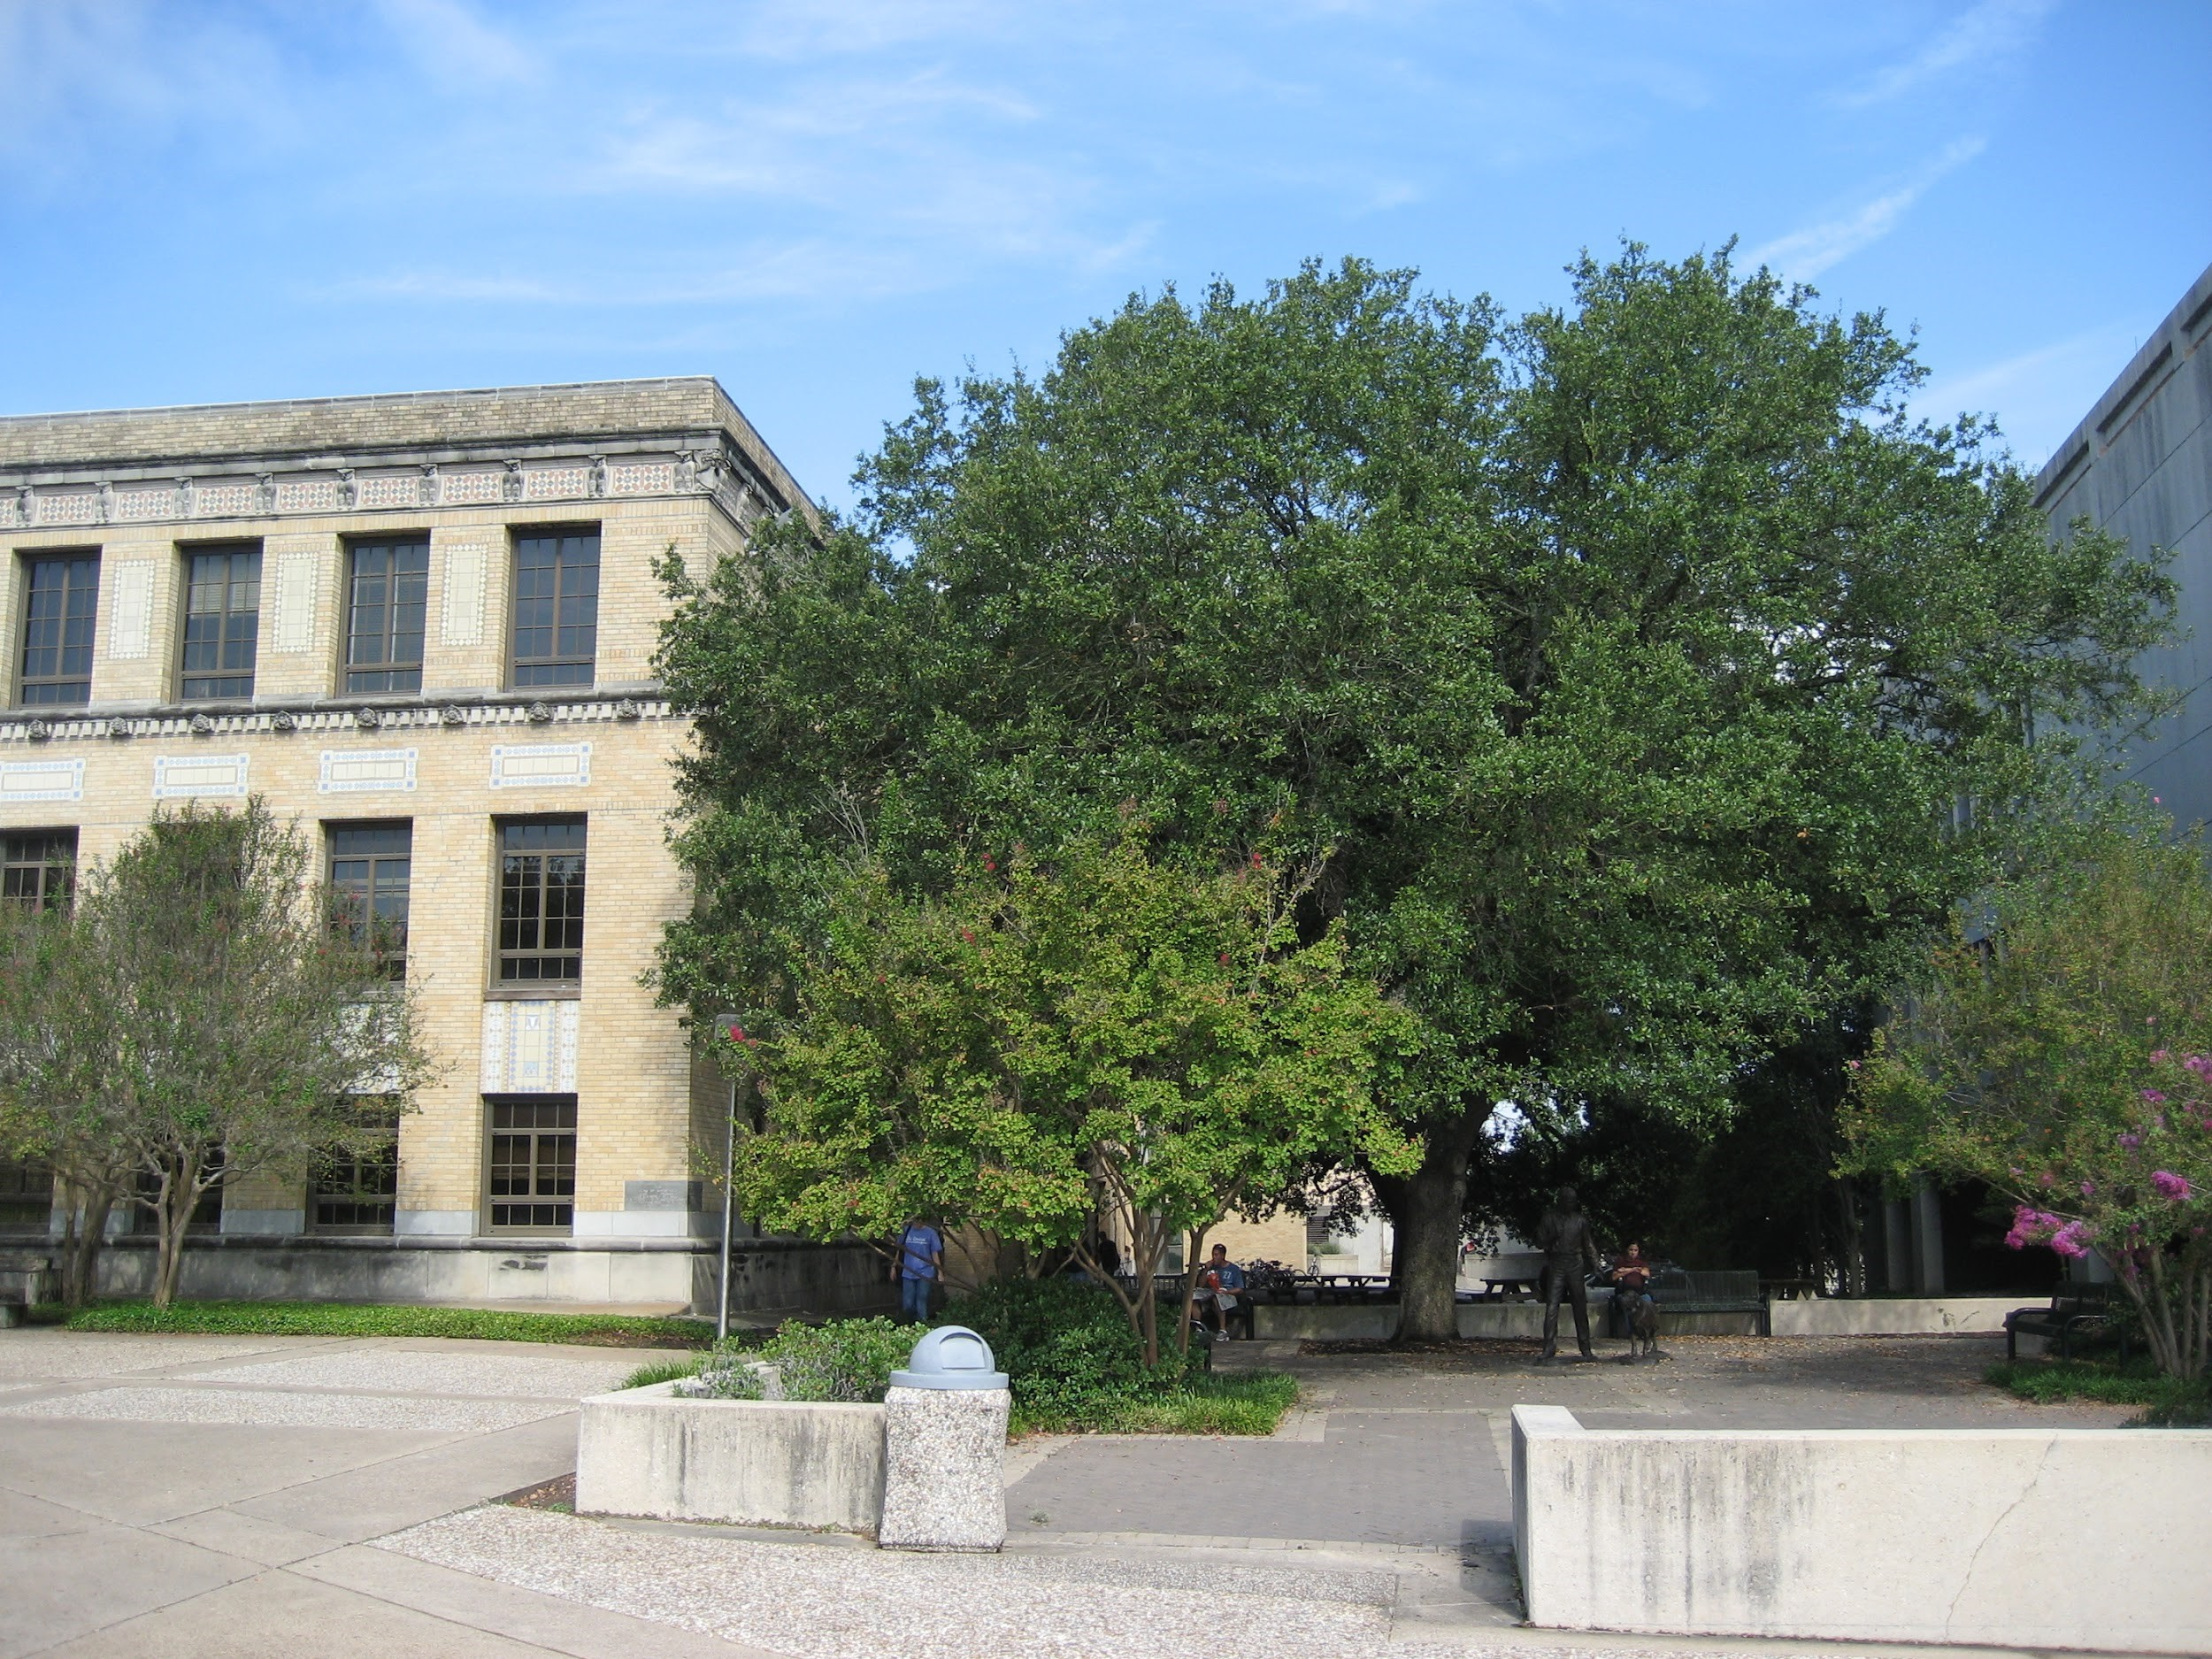
\includegraphics[width=0.49\linewidth]{fig_2.jpg}}
%  \caption{Original images}
%  \label{org_img} %% label for entire figure
%\end{figure*}

%\begin{figure}[htbp]
%\begin{center}
%\includegraphics[width=\linewidth]{pure_dlt.jpg} 
%\end{center}	   
%\caption{Panorama formed by result of pure DLT}\label{pure_dlt}
%\end{figure}

\section{Camera Calibration}
Recall from projects before, we have implemented DLT approach for finding the transformation homography from one image to another. Now in the camera calibration process, we can use similar methods, let's first review the original DLT approach and normalization process. 
\subsection{DLT Foundation}
In the simplest DLT approach, we first transform the homogeneous equation given in equation 7 as follows:
\begin{equation}
	\mat{x}_i \times \mat{P}\mat{X}_i = \mat{0}
\end{equation}
Where $\mat{P}$ is the camera matrix and can be decomposed into combination of vectors like:
\begin{equation}
	\mat{P} = \begin{pmatrix}
				\mat{p_1}\\
				\mat{p_2}\\
				\mat{p_3}
		       \end{pmatrix}
\end{equation}
Then we can rewrite equation 7 into the following form:
\begin{equation}
	\mat{P}\mat{X}_i =
	\begin{pmatrix}
		\mat{p}_1\mat{X}_i\\
		\mat{p}_2\mat{X}_i\\
		\mat{p}_3\mat{X}_i
	\end{pmatrix}
\end{equation}
Suppose the coordinates of the set of points we have are:
\begin{equation}
	\begin{split}
		\mat{x}_i = (x_i, y_i, z_i)
	\end{split}
\end{equation}
As we have $\mat{p}_i\mat{X}_i = \mat{X}_i^T \mat{p}_j^T$, we can further get the following simultaneous linear equations set:
\begin{equation}
	\begin{bmatrix}
		\mat{0}^T & -z_i\mat{X}_i^T & y_i\mat{X}_i^T\\
		z_i\mat{X}_i^T & \mat{0}^T & -x_i\mat{X}_i^T\\
		-y_i\mat{X}_i^T & x_i\mat{X}_i^T & \mat{0}^T
	\end{bmatrix}
	\begin{pmatrix}
		\mat{p}_1^T\\
		\mat{p}_2^T\\
		\mat{p}_3^T
	\end{pmatrix} = \mat{0}
\end{equation}

Be noticed that different from the math we did before in last project, here $\mat{X}_i$ is a 4D coordinates and $p_i$ also contains 4 entries. 
Since we can obtain the 3rd row of the left matrix above using by combining first two rows up to scale, we can safely prune equation 7 to only preserve the linearly independent first two rows in that matrix and obtain:
\begin{equation}
	\mat{A}
	\mat{p} = \mat{0}
\end{equation}
where
\begin{equation}
	\mat{A} = 
	\begin{bmatrix}
		\mat{0}^T & -z_i\mat{X}_i^T & y_i\mat{X}_i^T\\
		z_i\mat{X}_i^T & \mat{0}^T & -x_i\mat{X}_i^T\\
		-y_i\mat{X}_i^T & x_i\mat{X}_i^T & \mat{0}^T
	\end{bmatrix},
	\mat{p} = 
	\begin{pmatrix}
		\mat{p}_1^T\\
		\mat{p}_2^T\\
		\mat{p}_3^T
	\end{pmatrix}
\end{equation}
As we know:
\begin{equation}
	\mat{P} = 
	\begin{pmatrix}
		\mat{p}_1\\
		\mat{p}_2\\
		\mat{p}_3
	\end{pmatrix}
	=
	\begin{bmatrix}
		p_1 & p_2 & p_3 & p_4\\
		p_5 & p_6 & p_7 & p_8\\
		p_9 & p_{10} & p_{11} & p_{12}
	\end{bmatrix}
\end{equation}

Now we have come to the point that is very similar to what we have done before in Project 1. After dehomogenization, the equation 12 we get is actually a equation with 11 unknowns in $\mat{p}$ (11 DoFs) which we can solve exactly if we have $5\frac{1}{2}$ point pairs (every point pair provide 2 equations), to get the homography we can do as the followings:
\begin{itemize}
	\item If we have exact $5\frac{1}{2}$ point correspondences (which means the we can only know one of the coordinate for sixth points) in both images, we can solve equation 12 to get an exact solution, but as there might be some noises in both images, it could lead to very bad results.
	\item We can also solve this equation is we can find more point correspondence to get so-called overdetermined solution through singular value decomposition (SVD), that way we should get more accurate results since we are provided with more information in the image.
\end{itemize}

\subsection{Normalized DLT}
\subsubsection{2D Image Frame Normalization}
Similar to the DLT part we did in finding transformation homography between two images, it's sometimes very important to carry out coordinates normalization to provide better homography (camera matrix in current case). $\mat{x}_i$ is in the same dimension as before, thus we can normalize it using previous method, i.e., the points should be translated so that centroid of all points is at the origin and we also need to scale them so that their RMS (root-mean-squared) distance from origin is $\sqrt{2}$. 
\subsubsection{3D World Frame Normalization}
However, with the introduction of points in world frame, we now have to consider the 3D points $\mat{X}_i$. To simplify the problem, here we consider the case where the variation in point depth from the camera is relatively slight we can do similar normalization for 3D points as we did for 2D points. Therefore, we translate centroid of all measured points to the origin and scale their coordinates so that RMS distance from the origin is $\sqrt{3}$. As mentioned in the textbook, such 2D-alike approach is actually suitable for a compact distribution of points.

\subsection{Camera Calibration Steps}
According to the textbook, the camera calibration steps can be carried out as shown in Figure \ref{calibrate_gold}.
\begin{figure*}
  \label{calibrate_gold}
  \centering \includegraphics{calibration_gold.png}
  \caption{Algorithm of Camera Calibration using Gold Standard}
\end{figure*}

%\newpage
%\appendix
%\subsection{Main Entry}
%\lstinputlisting{codes/hw2.m}
% conference papers do not normally have an appendix


% use section* for acknowledgment





% trigger a \newpage just before the given reference
% number - used to balance the columns on the last page
% adjust value as needed - may need to be readjusted if
% the document is modified later
%\IEEEtriggeratref{8}
% The "triggered" command can be changed if desired:
%\IEEEtriggercmd{\enlargethispage{-5in}}

% references section

% can use a bibliography generated by BibTeX as a .bbl file
% BibTeX documentation can be easily obtained at:
% http://mirror.ctan.org/biblio/bibtex/contrib/doc/
% The IEEEtran BibTeX style support page is at:
% http://www.michaelshell.org/tex/ieeetran/bibtex/
%\bibliographystyle{IEEEtran}
% argument is your BibTeX string definitions and bibliography database(s)
%\bibliography{IEEEabrv,../bib/paper}
%
% <OR> manually copy in the resultant .bbl file
% set second argument of \begin to the number of references
% (used to reserve space for the reference number labels box)
%\bibliographystyle{IEEEtran}
% argument is your BibTeX string definitions and bibliography database(s)
%\bibliography{refs}




% that's all folks
\end{document}


